\documentclass{beamer}

\mode<presentation> {
\usetheme{Boadilla}
\usecolortheme{default}
}
%\usepackage{natbib}
\usepackage{amsmath}
\usepackage{amssymb}
\usepackage{amsthm}
\usepackage{bibentry}
\usepackage{graphicx} % Allows including images
\usepackage{booktabs} % Allows the use of \toprule, 
\usepackage{listings}
\usepackage{minted}

\title[CodeSeoul] % (optional, only for long titles)
	{Optimization algorithms in deep learning}

\author[AI Research Paper Review] % (optional, for multiple authors)
	{Sanzhar Askaruly}

\institute[] % (optional)
	{ Ulsan National Institute of Science and Technology\newline
	  Ph.D. Candidate in Biomedical Engineering}

\date{\today} 

% some change
\begin{document}
    %\maketitle
    % \begin{frame}
    % \titlepage % Print the title page as the first slide
    % \end{frame}

    \begin{frame}
    \frametitle{Overview} % Table of contents slide, comment this block out to remove it
    \tableofcontents 
    \end{frame}

    \begin{frame}
      \frametitle{Stochastic Gradient Descent (SGD)} % Table of contents slide, comment this block out to remove it
      \begin{block}{Algorithm}
        Update step:
        \begin{equation}    % <--- deleted empty lines
          \theta_{t+1} = \theta_{t} - \eta \cdot \nabla_{\theta}J(\theta_t)
        \end{equation}
      \end{block}
    \end{frame}

    \begin{frame}
      \frametitle{SGD with Momentum} % Table of contents slide, comment this block out to remove it
      \begin{block}{Algorithm}
        Update step:
        \begin{equation}    % <--- deleted empty lines
          v_{t,i} = \gamma \cdot v_{t-1,i} + \nabla_{\theta}J(\theta_{t,i})
        \end{equation}
        \begin{equation}    % <--- deleted empty lines
          \theta_{t+1} = \theta_{t} - \eta \cdot v_{t,i}
        \end{equation}
      \end{block}
    \end{frame}

    \begin{frame}[fragile]
      \frametitle{Optimizers in PyTorch}

      Vanilla training loop in \verb|PyTorch|:
      \rule{\textwidth}{1pt}
      \scriptsize
      \begin{minted}{python}
          for input, target in dataset:
            optimizer.zero_grad()
            output = model(input)
            loss = loss_fn(output, target)
            loss.backward()
            optimizer.step()
      \end{minted}
      \rule{\textwidth}{1pt}
      
      \normalsize
      \vspace{1cm}
      How to use an optimizer:
      \rule{\textwidth}{1pt}
      \scriptsize
      \begin{minted}{python}
        optimizer = optim.SGD(model.parameters(), lr=0.01, momentum=0.9)
        #optimizer = optim.Adam(model.parameters(), lr=0.0001)
      \end{minted}
      \rule{\textwidth}{1pt}
      

    \end{frame}

    \begin{frame}{First images in beamer}
      \centering
          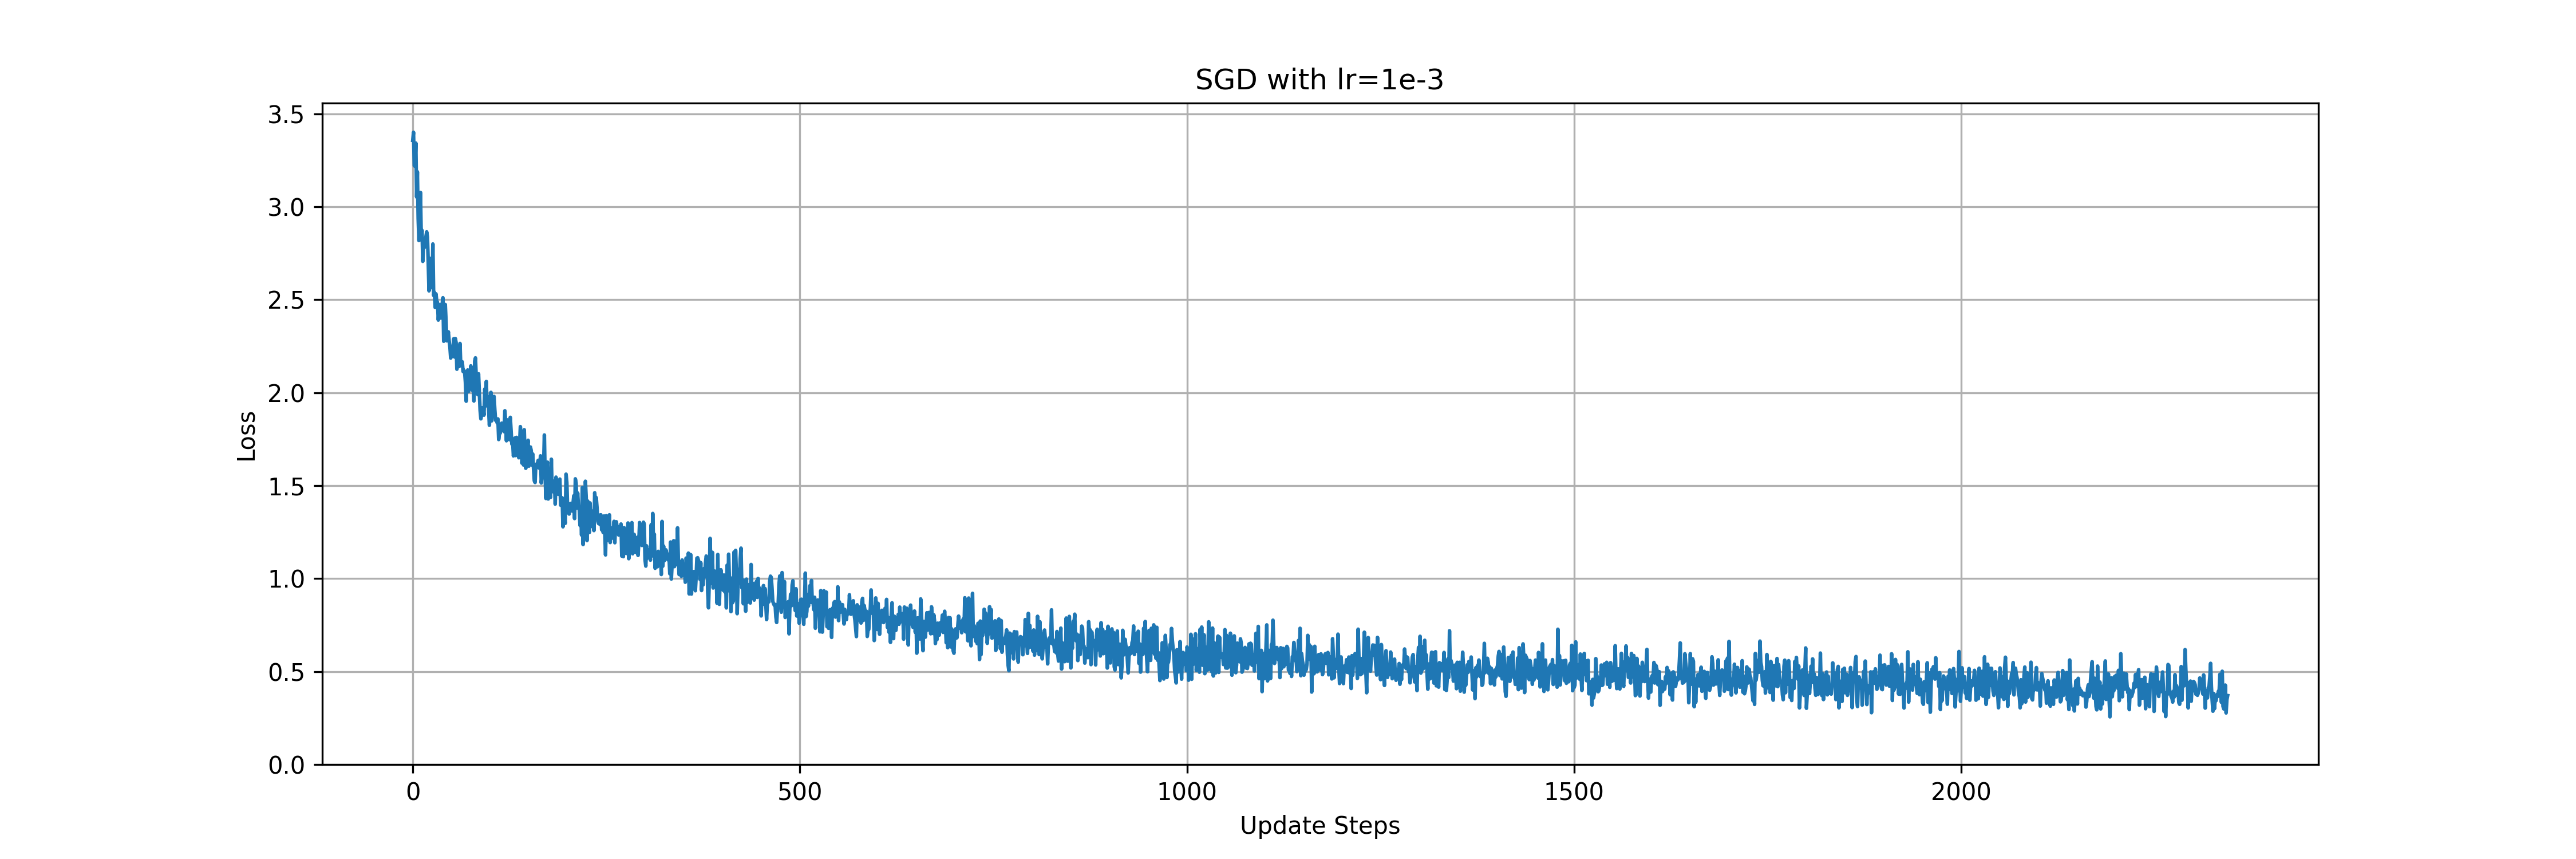
\includegraphics[scale=0.3]{/home/suzy/gitrepos/tuttelikz/221105/images/sgd.png}
    \end{frame}
    

    \begin{frame}[fragile] % Need to use the fragile option when verbatim is used in the slide
    \frametitle{Citation}
    An example of the \verb|\cite| command to cite within the presentation:\\~
    
    This statement requires citation.~\cite{test1} 
    \end{frame}

    

    \begin{frame}[t, allowframebreaks]
      \frametitle{References}
      \bibliographystyle{amsalpha}
      \bibliography{bibfile}
    \end{frame}

\end{document}